\begin{frame}
  Linux Weekly News
  \frametitle{Kernel Development News}
  \begin{itemize}
  \item \url{http://lwn.net/}
  \item The weekly digest off all Linux and free software
    information sources
  \item In depth technical discussions about the kernel
  \item Subscribe to finance the editors (\$7 / month)
  \item Articles available for non subscribers after 1 week.
  \end{itemize}
\end{frame}

\begin{frame}
  \frametitle{Useful Reading (1)}
  \begin{columns}
    \column{0.7\textwidth}
    Essential Linux Device Drivers, April 2008
    \begin{itemize}
    \item \url{http://elinuxdd.com/}
    \item By Sreekrishnan Venkateswaran, an embedded IBM engineer
      with more than 10 years of experience
    \item Covers a wide range of topics not covered by LDD: serial
      drivers, input drivers, I2C, PCMCIA, PCI,
      USB, video drivers, audio drivers, block drivers, network
      drivers, Bluetooth, IrDA, MTD, drivers in user space, kernel
      debugging, etc.
    \item \emph{Probably the most wide ranging and complete Linux
          device driver book I've read} -- Alan Cox
    \end{itemize}
    \column{0.3\textwidth}
    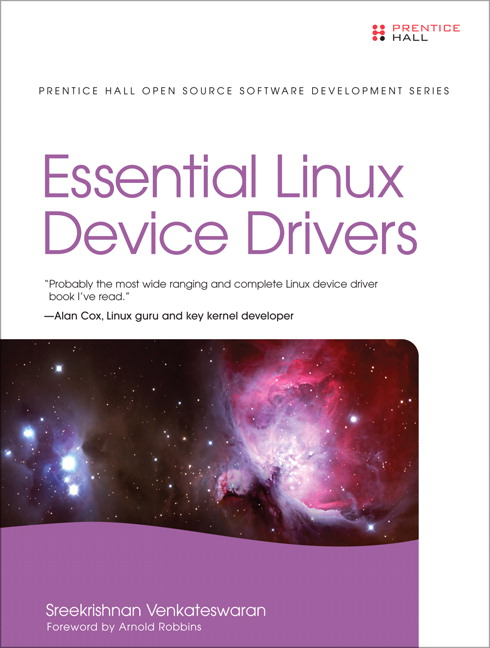
\includegraphics[width=\textwidth]{slides/kernel-resources-references/eldd.jpg}
  \end{columns}
\end{frame}

\begin{frame}
  \frametitle{Useful Reading (2)}
  \begin{columns}
    \column{0.7\textwidth}
    \begin{itemize}
    \item Linux Kernel Development, 3rd Edition, Jun 2010
      \begin{itemize}
      \item Robert Love, Novell Press
      \item \url{http://bootlin.com/redir/lkd3-book.html}
      \item A very synthetic and pleasant way to learn about kernel
        subsystems (beyond the needs of device driver writers)
      \end{itemize}
    \item The Linux Programming Interface, Oct 2010
      \begin{itemize}
      \item Michael Kerrisk, No Starch Press
      \item \url{http://man7.org/tlpi/}
      \item A gold mine about the kernel interface and how to use it
      \end{itemize}
    \end{itemize}
    \column{0.3\textwidth}
    \begin{center}
      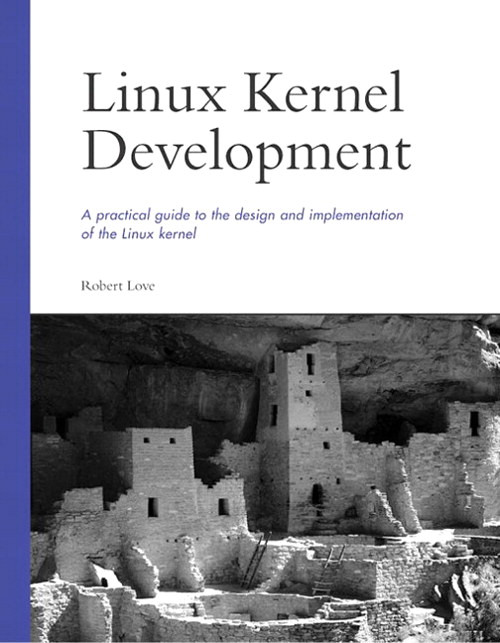
\includegraphics[height=0.4\textheight]{slides/kernel-resources-references/linux-kernel-development.jpg}\\
      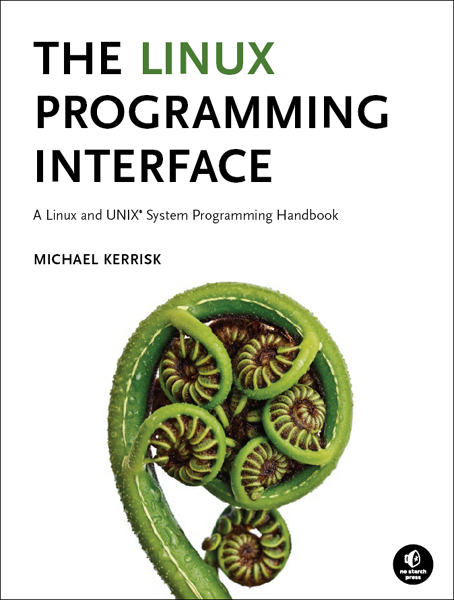
\includegraphics[height=0.4\textheight]{slides/kernel-resources-references/linux-programming-interface.png}
    \end{center}
  \end{columns}
\end{frame}

\begin{frame}
  \frametitle{Useful Online Resources}
  \begin{itemize}
  \item Kernel documentation
    \begin{itemize}
    \item \url{https://kernel.org/doc/}
    \end{itemize}
  \item Linux kernel mailing list FAQ
    \begin{itemize}
    \item \url{http://vger.kernel.org/lkml/}
    \item Complete Linux kernel FAQ
    \item Read this before asking a question to the mailing list
    \end{itemize}
  \item Kernel Newbies
    \begin{itemize}
    \item \url{http://kernelnewbies.org/}
    \item Glossary, articles, presentations, HOWTOs, recommended
      reading, useful tools for people getting familiar with Linux
      kernel or driver development.
    \end{itemize}
  \item Kernel glossary
    \begin{itemize}
    \item \url{http://kernelnewbies.org/KernelGlossary}
    \end{itemize}
\end{itemize}

\end{frame}

\begin{frame}
  \frametitle{International Conferences}
  \begin{itemize}
  \item Embedded Linux Conference:
    
\includegraphics[width=0.35\textwidth]{slides/kernel-resources-references/elc-logo.png}\\
    \url{http://embeddedlinuxconference.com/}
    \begin{itemize}
    \item Organized by the Linux Foundation in the USA (February-April)
          and in Europe (October-November)
    \item Very interesting kernel and user space topics for embedded
      systems developers.
    \item Presentation slides and videos freely available
    \end{itemize}
  \item Linux Plumbers: \url{http://linuxplumbersconf.org}
    \begin{itemize}
    \item Conference on the low-level plumbing of Linux: kernel,
      audio, power management, device management, multimedia, etc.
    \end{itemize}
  \item linux.conf.au: \url{http://linux.org.au/conf/}
    \begin{itemize}
    \item In Australia / New Zealand
    \item Features a few presentations by key kernel hackers.
    \end{itemize}
  \end{itemize}
\end{frame}

\begin{frame}
  \frametitle{Continue to learn after the course}
  Here are a few suggestions:
  \begin{itemize}
  \item Run your labs again on your own hardware. The Nunchuk lab should
        be rather straightforward, but the serial lab will be quite different
	if you use a different processor.
  \item Help with tasks keeping the kernel code clean and up-to-date:\\
	\url{http://kernelnewbies.org/KernelJanitors}
  \item Propose fixes for issues reported by the {\em Coccinelle} tool:\\
	\code{make coccicheck}
  \item Learn by reading the kernel code by yourself, ask questions and
	propose improvements.
  \item Implement and share drivers for your own hardware, of course!
  \end{itemize}
\end{frame}
